\documentclass{beamer}
\usepackage[utf8]{inputenc}
\usepackage{xcolor}
\usepackage{listings}
\usepackage{graphicx}
\usetheme[secheader]{Boadilla}
\definecolor{coultitre}{rgb}{0,0.65,0}
\setbeamercolor{structure}{fg=coultitre, bg=coultitre!40} 


\title{Vidéo surveillance, Streaming vidéo et contrôle de caméra via Android }
\author{Jérôme NAHELOU, Quentin NEBOUT, Romain SOLVE,\\Fabien QUINTARD}
\institute{\large{Chargé de Projet : Yérom-David Bromberg}\\ \bigskip{}
\small{Université Bordeaux 1}}
\date{29 mars 2011}

\begin{document}
\frame[plain]{
\includegraphics[scale=0.20]{logo-bdx1.pdf}\titlepage}

\AtBeginSection[]{
\begin{frame}<beamer>
\frametitle{Plan}
\small{\tableofcontents[currentsection,hideallsubsections]}
\end{frame}}

\begin{frame}
\frametitle{Plan de l'exposé}
\small{\tableofcontents[hideallsubsections]}
\end{frame}

  \begin{frame}
   \frametitle{Description}
  Introduction
  % schéma projet : dessin camera + portablets et tablettes android en réseau %
   \begin{itemize}
    \item Android: OS pour appareil mobile, basé sur noyaux linux
    \item Choix: M-JPEG, HTTP-GET
   \end{itemize}
  \end{frame}
  
  %\begin{frame}
   %\frametitle{Besoins}
  %Introduction%
  % schéma besoins F / besoins NF 
  %\end{frame}
 

\section{Aspect général de l'application}
  \subsection{Description}
  \begin{frame}
   \frametitle{Description de l'application}
   \begin{itemize}
   \item Fonctionnement sous Android
       \begin{itemize}
    	\item Téléphone mobile
   		\item Tablette tactile
    	\end{itemize}
   \item Réservée aux caméras de la marque Axis
   		\begin{itemize}
    	\item Compatible pour tout les modèles
   		\item Intègration des fonctions propres au caméra
    	\end{itemize}
   \item Facilité d'utilisation
   		\begin{itemize}
    	\item Sauvegarde de profil utilisateur
   		\item Traduit pour plusieurs langues
    	\end{itemize}
   \end{itemize}
  \end{frame}


%\section{Simple vue}
%\subsection{Spécifications}
% \begin{frame}
%   \frametitle{Spécifications}
%   \begin{itemize}
%    \item Réutilisation d'un lecteur MJPEG existant : MjpegView
%    \item Interface de contrôle de la caméra
%    % screen simple vue %
%    \end{itemize}
%\end{frame}

%\section{Multi-vue}
%\subsection{Spécifications}
% \begin{frame}
%   \frametitle{Spécifications}
%   \begin{itemize}
%    \item Implémentation de layouts personnalisés pour 2 à 6 caméras
%    % schéma ou screen multi-vue %
%    \item Rafraîchissement multi-threadé (un thread par caméra)
%    % schéma UML de Jérôme ;) %
%    \item Ajout de listeners pour gérer les caméras et passer en simple vue 
%    \end{itemize}
%\end{frame}

%\section{Contrôle de la caméra}
%\subsection{Implémentation}
% \begin{frame}
%   \frametitle{Implémentation}
%   \begin{itemize}
%    \item Communication avec la caméra par requêtes HTTP
%    \item Chargement de la configuration à l'initialisation de la vidéo
%    \item Méthode de construction et d'envoi des requêtes avec
%    authentification et délai variable de connexion
%   \end{itemize}
%\end{frame}



\subsection{Besoins}
  \begin{frame}
   \frametitle{Besoins pour l'application}

  \centering
  \begin{minipage}{0.95\textwidth}
	\begin{itemize}
    \item Besoins fonctionels de l'application
    \end{itemize}
    \end{minipage}
   
     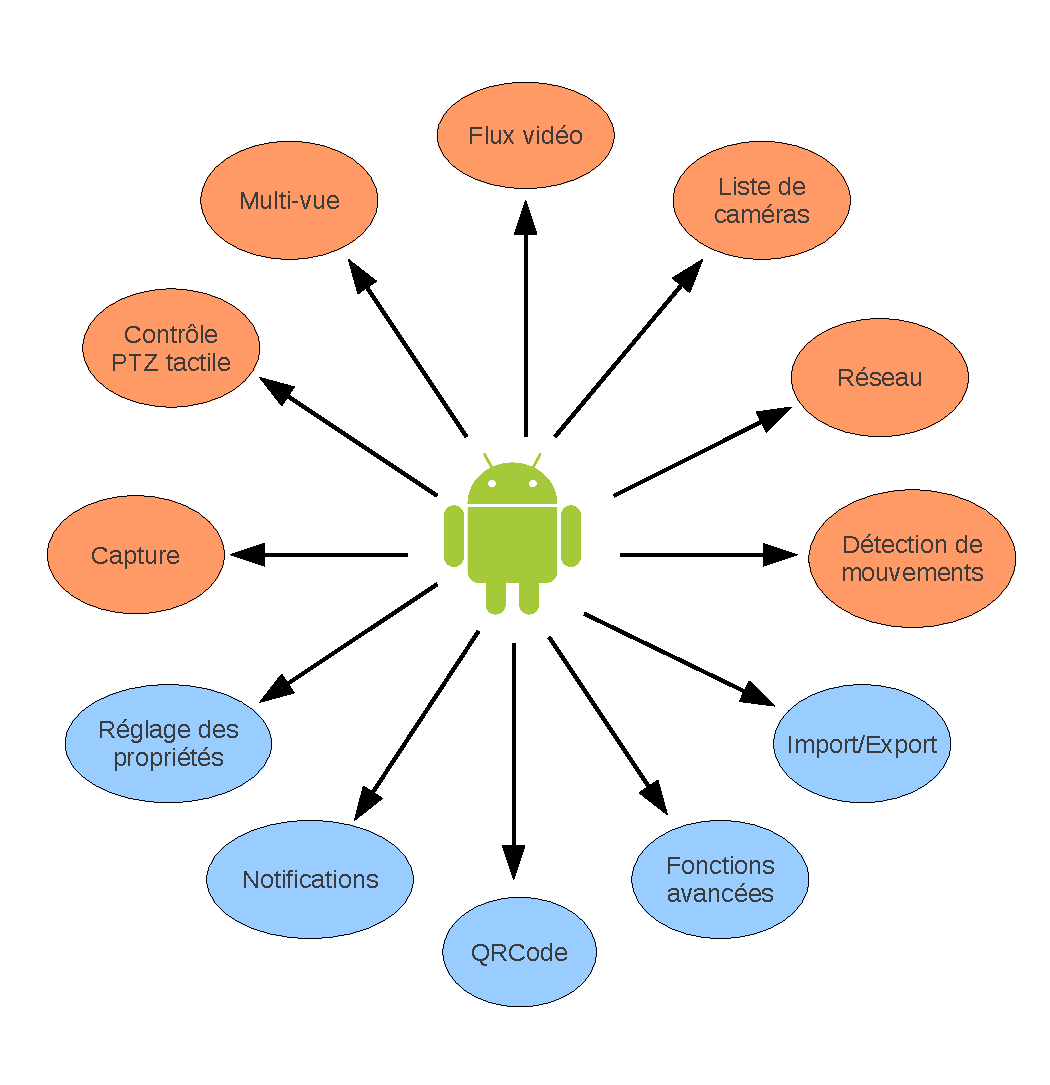
\includegraphics[scale=0.4]{Images/besoinsF.pdf}
   
  \end{frame}

\subsection{Besoins}
  \begin{frame}
   \frametitle{Besoins pour l'application}

  \centering
  \begin{minipage}{0.95\textwidth}
	\begin{itemize}
    \item Besoins non fonctionels de l'application
    \end{itemize}
    \end{minipage}
   
     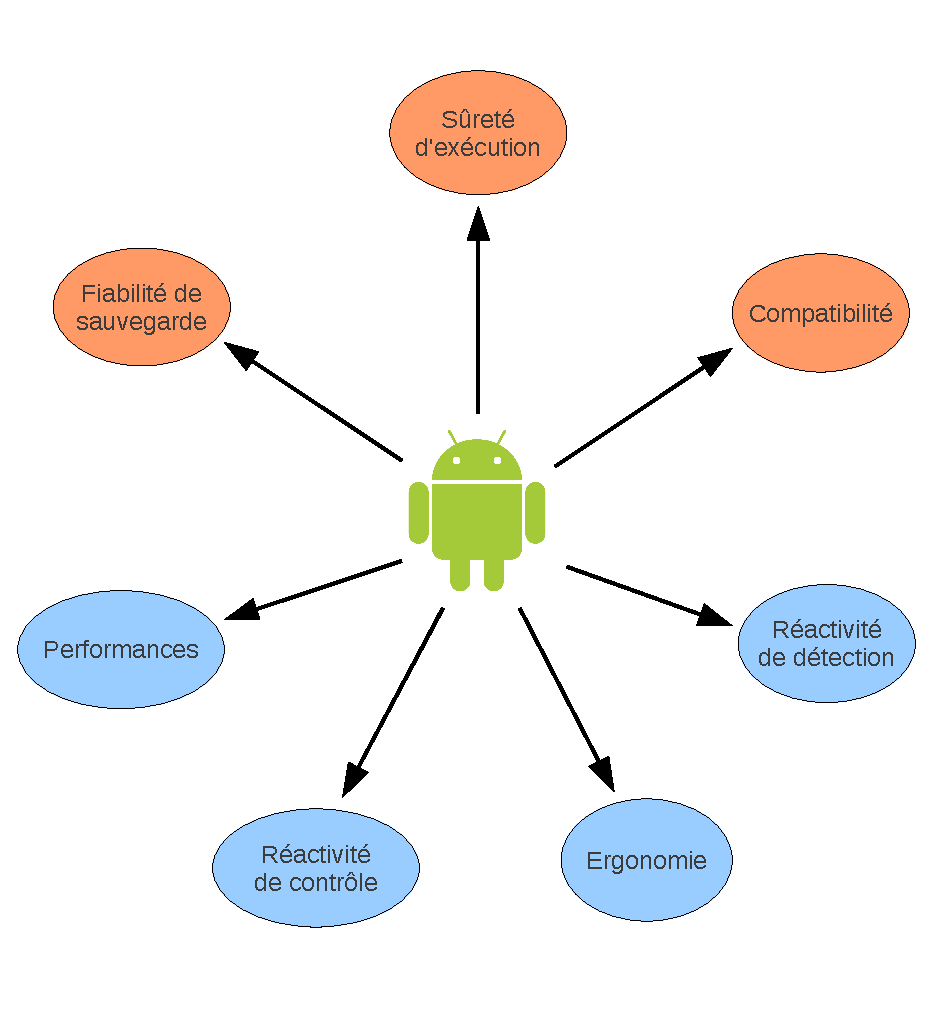
\includegraphics[scale=0.4]{Images/besoinsNF.pdf}
   
  \end{frame}

\section{Gestion des caméras}
  \begin{frame}
   \frametitle{Gestion des caméras}


\begin{figure}[H]
  \centering
  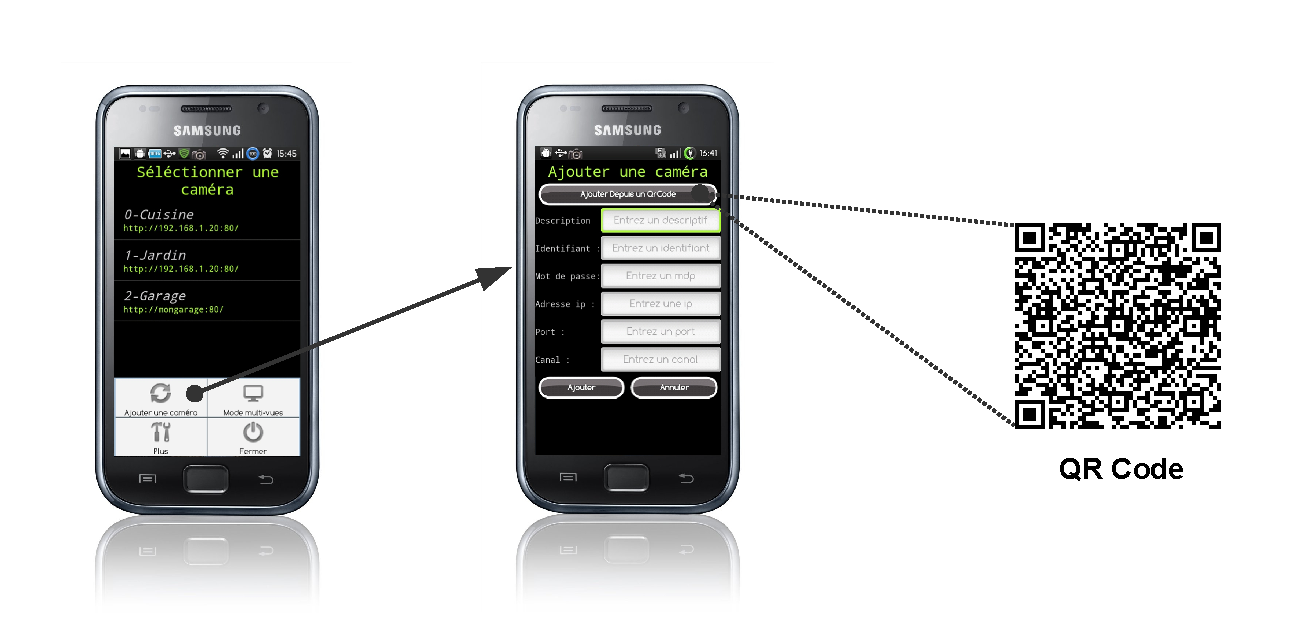
\includegraphics[scale=0.25]{Images/ImageSlide5.pdf}
     \begin{itemize}
    \item Ecran d'accueil de l'application, accès aux différentes activités
    \item Liste illimitée de caméras sauvegardable
    \item Gestion complète des caméras : ajout / édition / suppression
    \item Possiblité d'ajout par QRCode
   \end{itemize}
  \end{figure}  

  \end{frame}


\section{Simple vue}
  \begin{frame}
   \frametitle{Simple vue}


\begin{figure}[H]
  \centering
     \begin{enumerate}
    \item Visualisation de base (contrôle PTZ tactile)
    \item Interface de contrôles avancés
    \item Mode détection de mouvements
   \end{enumerate}
   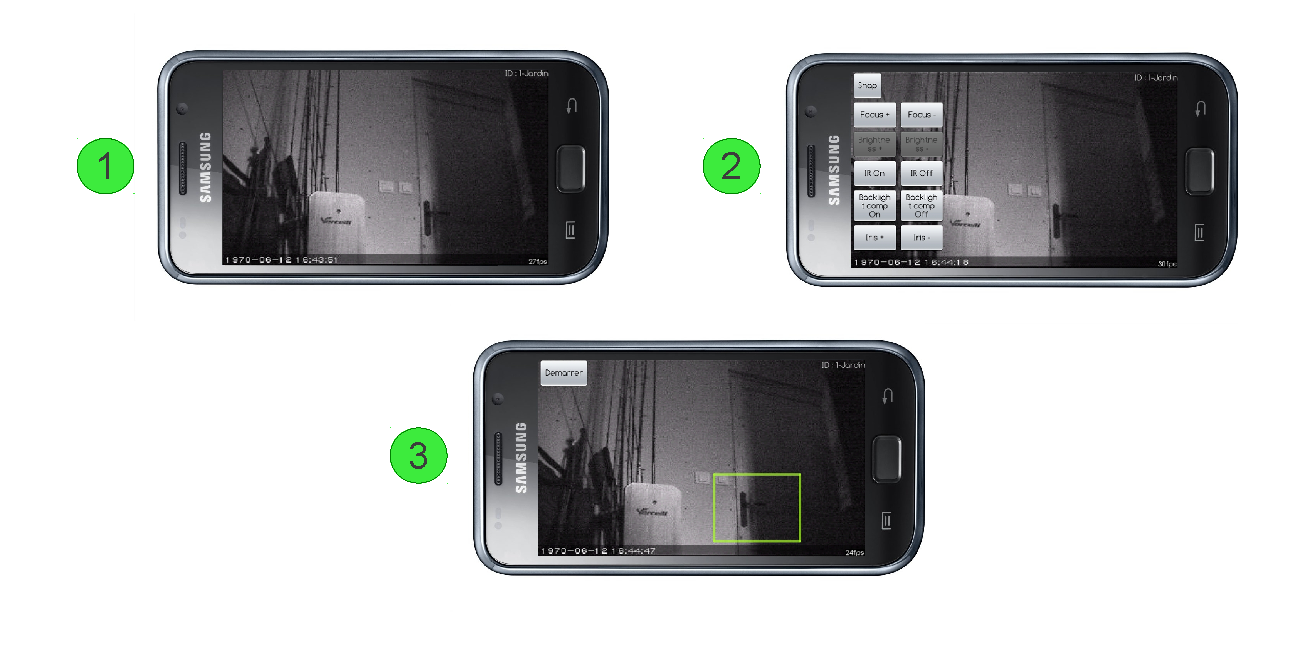
\includegraphics[scale=0.25]{Images/ImageSlide6.pdf}
  \end{figure}  

  \end{frame}

\section{Contrôle de la caméra}
\subsection{Communication avec la caméra}
  \begin{frame}
   \frametitle{Communication et configuration}

  \begin{minipage}{0.94\textwidth}
  \centering
     \begin{itemize}
    \item Classe dédiée au traitement des requêtes HTTP envoyées à la caméra
    \begin{itemize}
      \item Codes réponses divers
      \item Parsage si nécessaire
      \newline
    \end{itemize}
    \item Chargement de la configuration et des fonctionnalités supportées
    \begin{itemize}
      \item PTZ, focus, iris, luminosité, \ldots
      \item Mode auto, résolutions d'image
      \item Audio, détection de mouvements
      \newline
    \end{itemize}
    \item Adaptation de l'interface aux différents modèles de caméra Axis
    \begin{itemize}
      \item Etat des boutons
      \item Choix de la résolution pour la capture
      \newline
    \end{itemize}
   	\end{itemize}
  \end{minipage}

  \end{frame}

\subsection{Contrôle PTZ tactile}
  \begin{frame}
   \frametitle{Contrôle PTZ tactile}

  \centering
  \begin{minipage}{0.85\textwidth}
    \begin{itemize}
      \item Gestion du Pan-Tilt de la caméra  avec 1 pointeur
      (1)
      \item Gestion du Zoom avec 2 pointeurs (2)
      \item Réglage de la sensibilité dans les paramètres
   	\end{itemize}
   	\end{minipage}
   	
   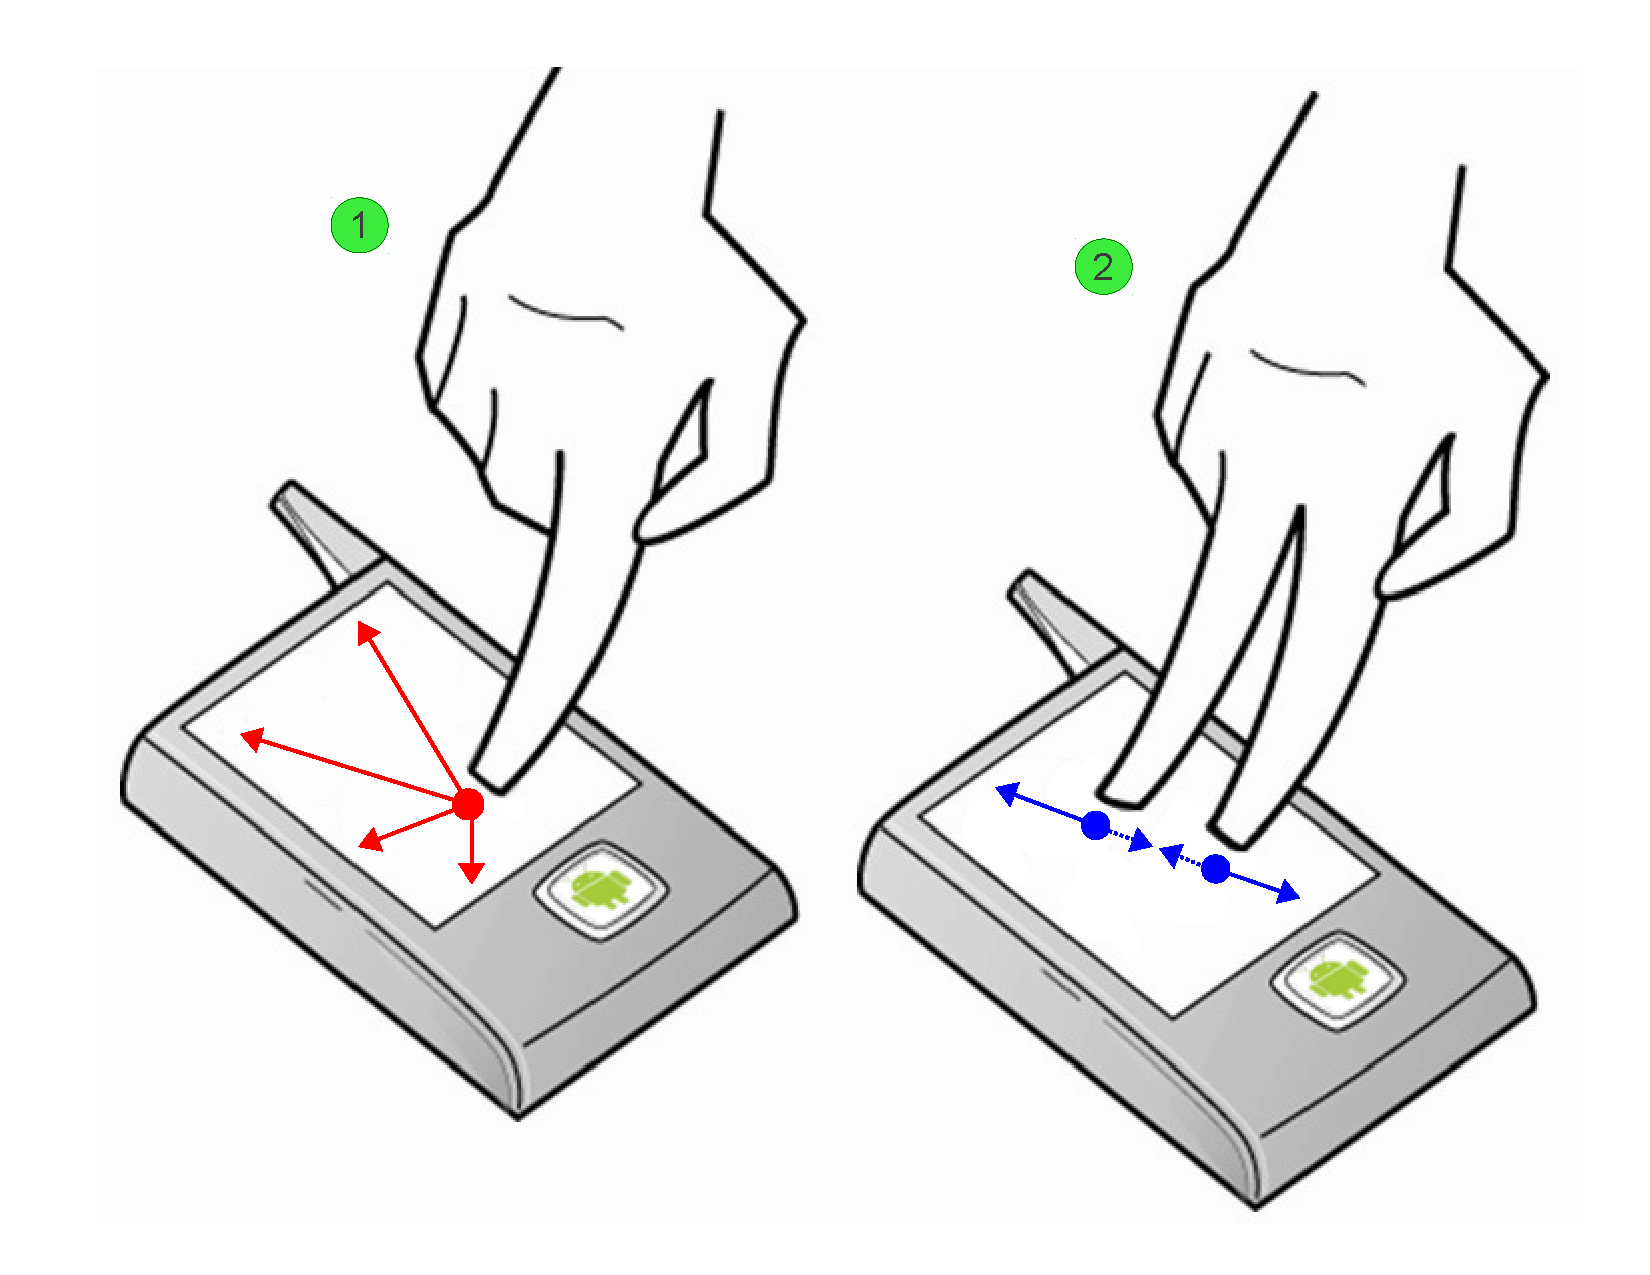
\includegraphics[scale=0.48]{Images/ImageSlide8.pdf}

  \end{frame}


\section{Vue Multiple}
  \subsection{Analyse du besoin}
  \begin{frame}
   \frametitle{Analyse du besoin}


\begin{figure}[H]
  \centering
  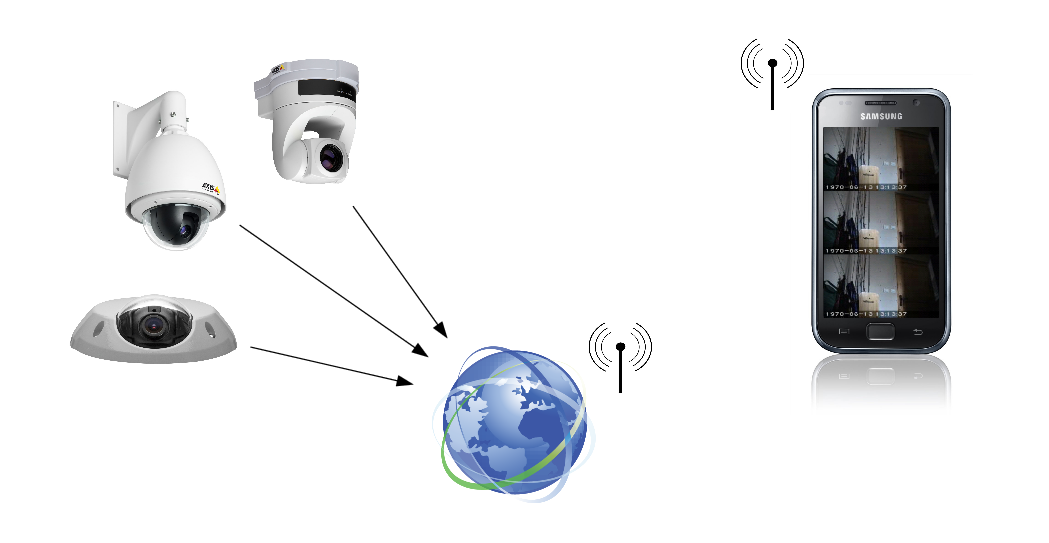
\includegraphics[scale=0.25]{Images/ImageSlide9.png}
     \begin{itemize}
    \item Possibilité de visionner 1 à 6 Caméras simultanément
    \item Choix de la disposition des caméras par l'utilisateur
    \item Réglage du nombre d'images par seconde
    \item Switch ``Multiple-Vue" - ``Vue unitaire"
   \end{itemize}
  \end{figure}  

\end{frame}

  \subsection{Utilisation et implémentation}
  \begin{frame}
   \frametitle{Utilisation}

\begin{columns}
\begin{column}{7cm}
\begin{enumerate}[<+->]
    \item Choix du mode d'affichage Multi-Vues
    \item Séléction du nombre de vue
  	\item Choix de l'emplacement
  	\item Choix de la caméra
  	\item Visualisation de la caméra
  	\item Un clic long permet la visualisation et le controle de la caméra dans
  	la vue simple
\end{enumerate}
\end{column}
\begin{column}{6cm}
  \centering \includegraphics<1>[width=3cm]{Images/mvstep/s1.jpg}
  \centering \includegraphics<2>[width=3cm]{Images/mvstep/s2.jpg}
  \centering\includegraphics<3>[width=5cm]{Images/mvstep/s3.jpg}
  \centering \includegraphics<4>[width=5cm]{Images/mvstep/s4.jpg}
  \centering \includegraphics<5>[width=5cm]{Images/mvstep/s5.jpg}
  \centering \includegraphics<6>[width=5cm]{Images/mvstep/s6.jpg}
\end{column}
\end{columns}

  \end{frame}
 
  \begin{frame}
   \frametitle{Implémentation}
\centering 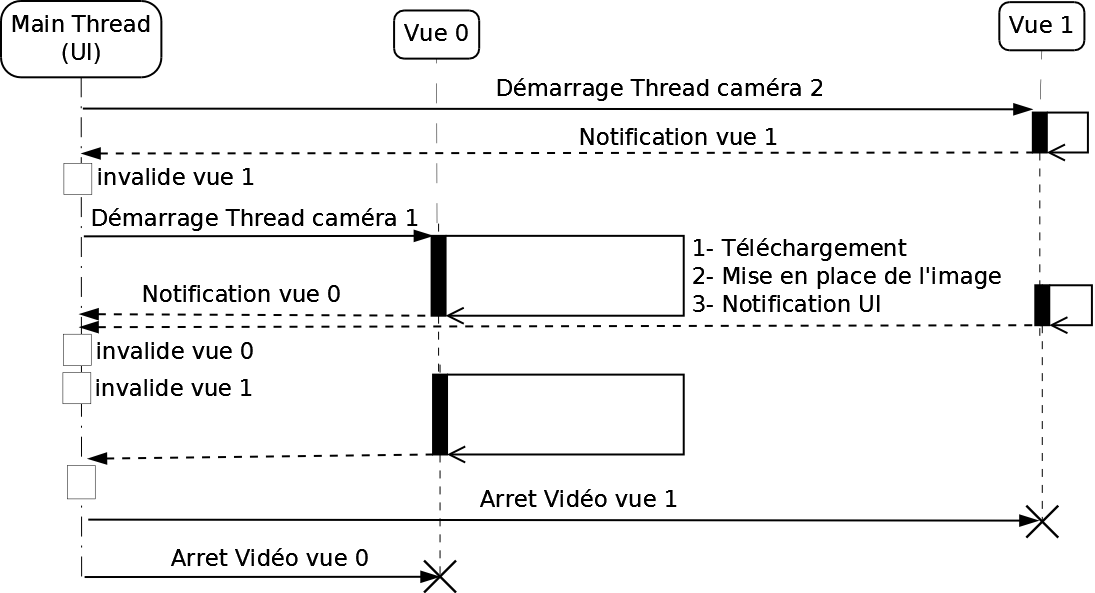
\includegraphics[scale=0.2]{Images/DiagrammeSequenceMultiView.png}

\begin{itemize}

    \item Chaque Thread notifie l'UI lorsqu'une nouvelle image est
    disponible
  	\item Délai réglable entre chaque début de téléchargement
  	\item Redessine uniquement la zone mise à jour
\end{itemize}
 \end{frame}
  

\section{Détection de mouvement}
 \subsection{Analyse du besoin}
  \begin{frame}
   \frametitle{Détection des mouvements :}



\begin{columns}
\begin{column}{5cm}

   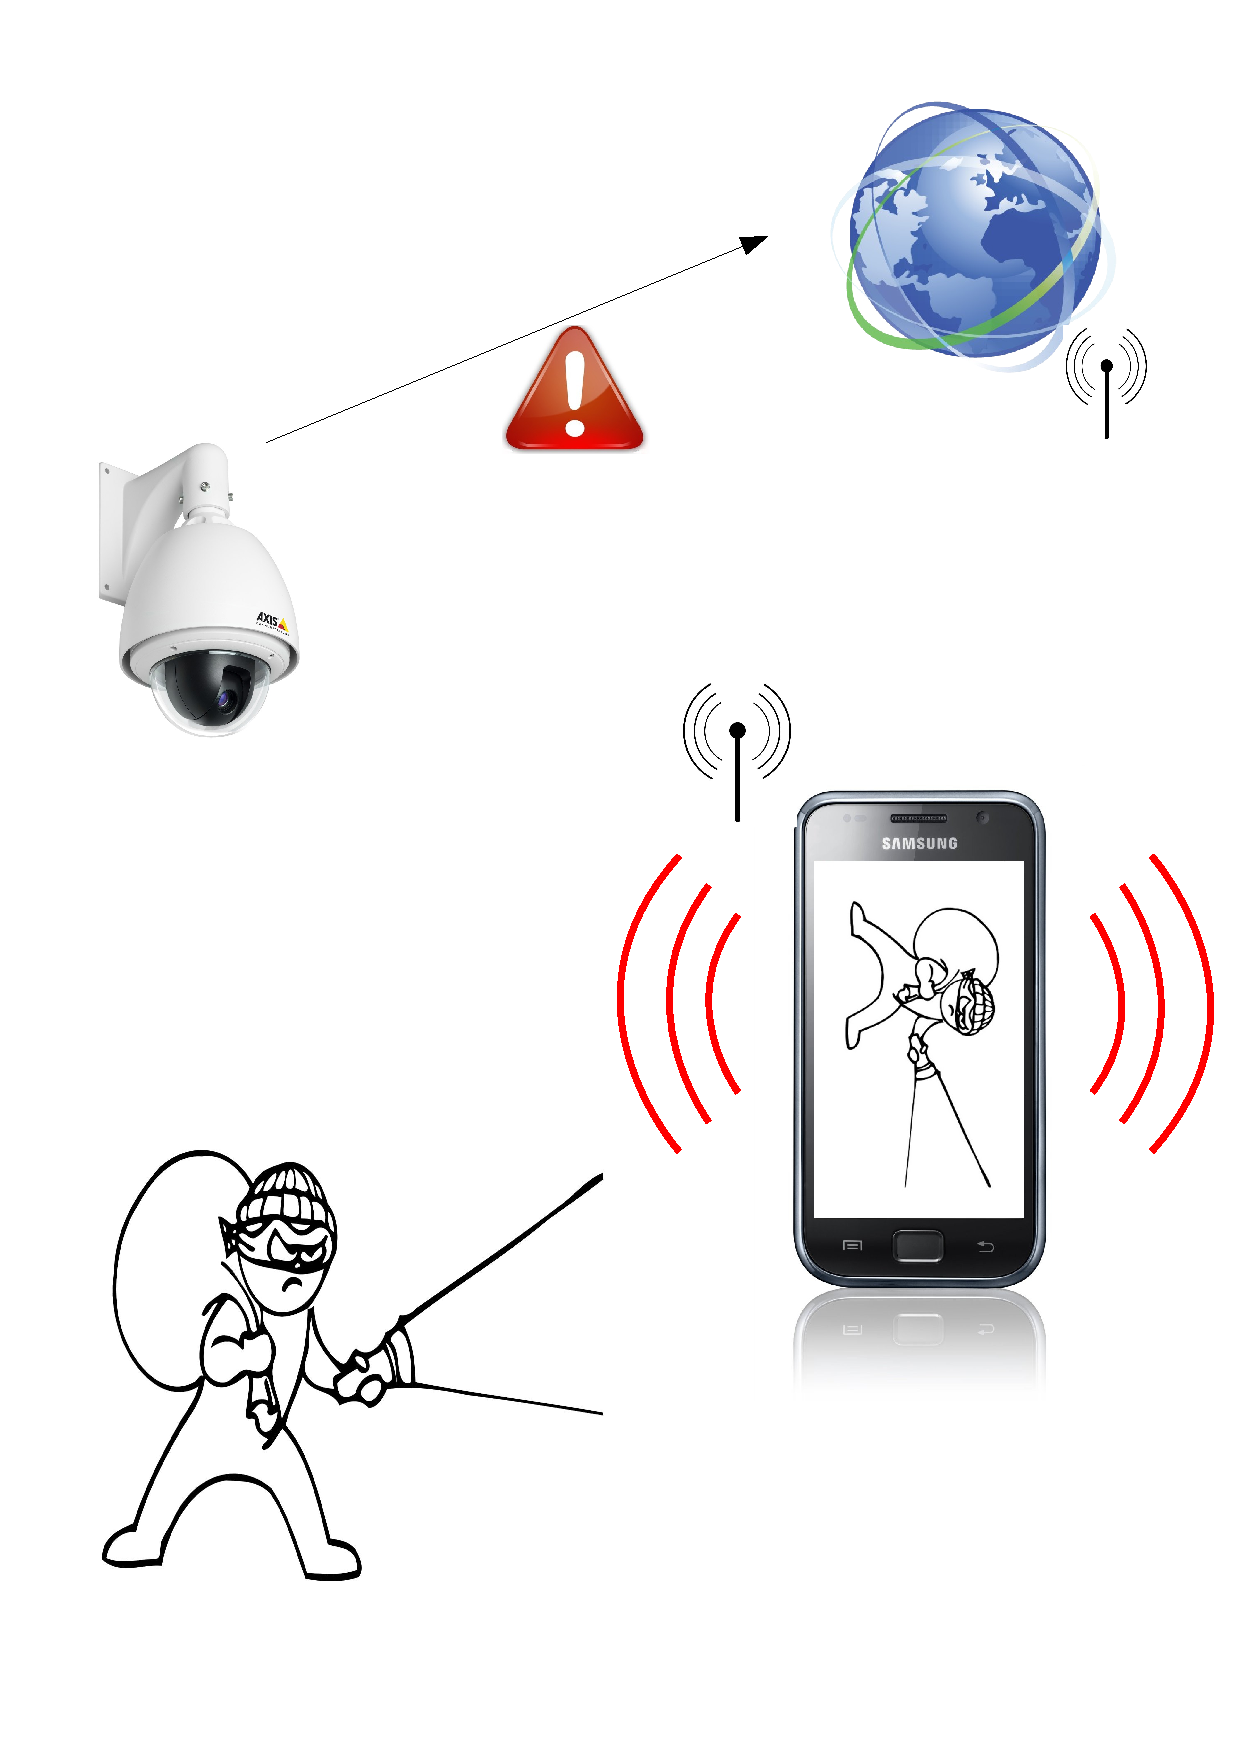
\includegraphics[scale=0.25]{Images/ImageSlide10.pdf}
\end{column}
\begin{column}{7cm}
\textbf{\textit{Caractéristiques :}} 
\begin{itemize}
    \item Réglage de la fenètre et du seuil de détection.
  	\item 1 à 10 fenètres par caméra.
  	\item Détection illimité pour des caméras differente.
 	\item Notification via Vibration et Cliché instantanné.
 	\item Utilisation facile et intuitive.
\end{itemize}
\end{column}
\end{columns}
  \end{frame}

  \subsection{Implémentation}
  \begin{frame}
   \frametitle{Procédure de lancement de la détection}
   Le traçage de la fenêtre par l'utilisateur (si nécessaire), puis un clic sur
   \newline le bouton démarrer entraîne :
   \begin{figure}[H]
 \centering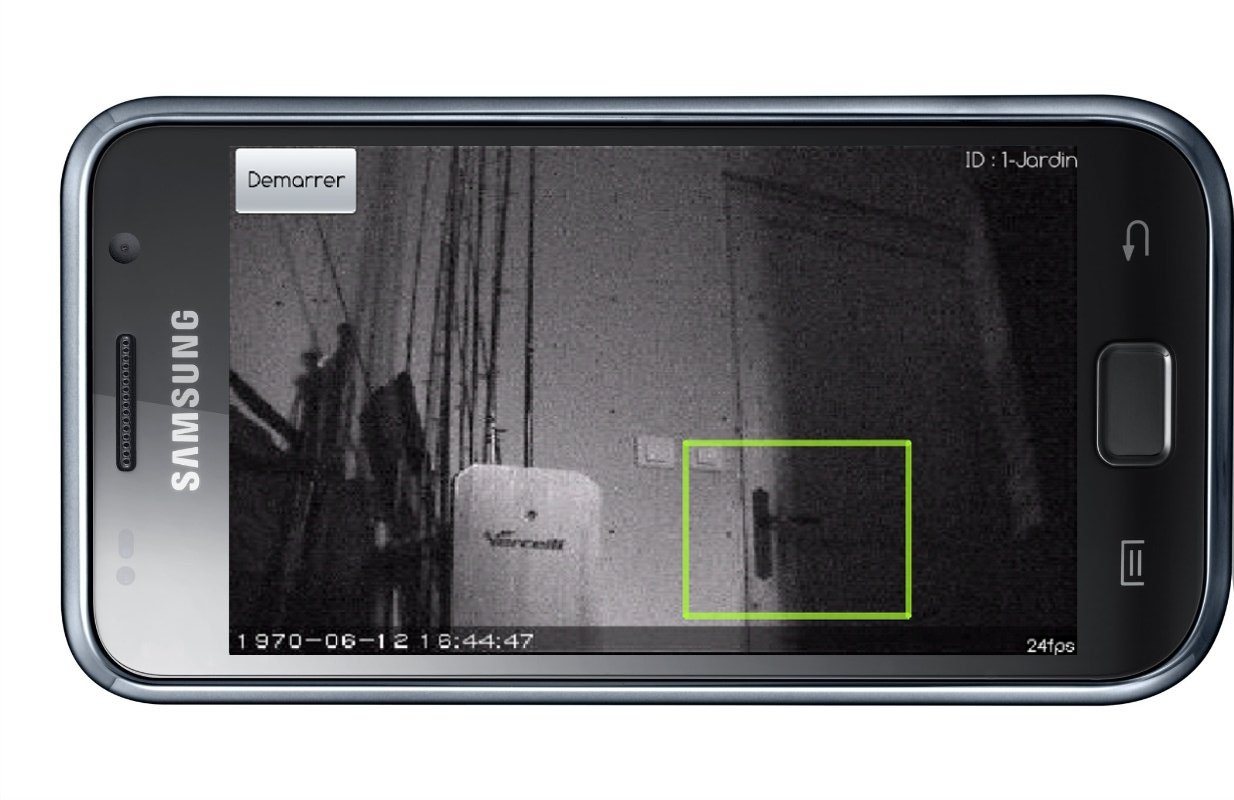
\includegraphics[scale=0.10]{Images/samsung-galaxy-s-vue3.jpg}
      \end{figure}
    \begin{enumerate}
    \item Demande d'ajout d'une fenêtre de détection auprès de la caméra
    \item Détéction de la présence d'une eventuelle fenêtre personnalisée puis
    mise à jour de ses coordonnées en cas de présence
    \item Démarrage de la tâche du service :
     \begin{enumerate}
       \item Ajout notification ``En-Cours''
       \item Démarrage d'un thread chargé d'analyser le niveau de détection
       retourné par la caméra
       \end{enumerate}
   \end{enumerate}
  \end{frame}
\section{Extras}
\begin{frame}
\frametitle{Extras}
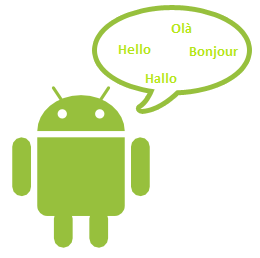
\includegraphics[width=3cm, height=2.5cm]{Images/ImageSlide11-3.png}\\
\begin{minipage}{0.69\textwidth}
\begin{itemize}
  \item Application Multi-langues
  \item Astuces au démarrage
  \item Prise de clichés instantanés (Snapshots)
  \item Partage de l'application et des caméras
  \item Import-export de la configuration
  \item Possibilité de générer la Javadoc 
\end{itemize}
\end{minipage}
\begin{minipage}{0.29\textwidth}
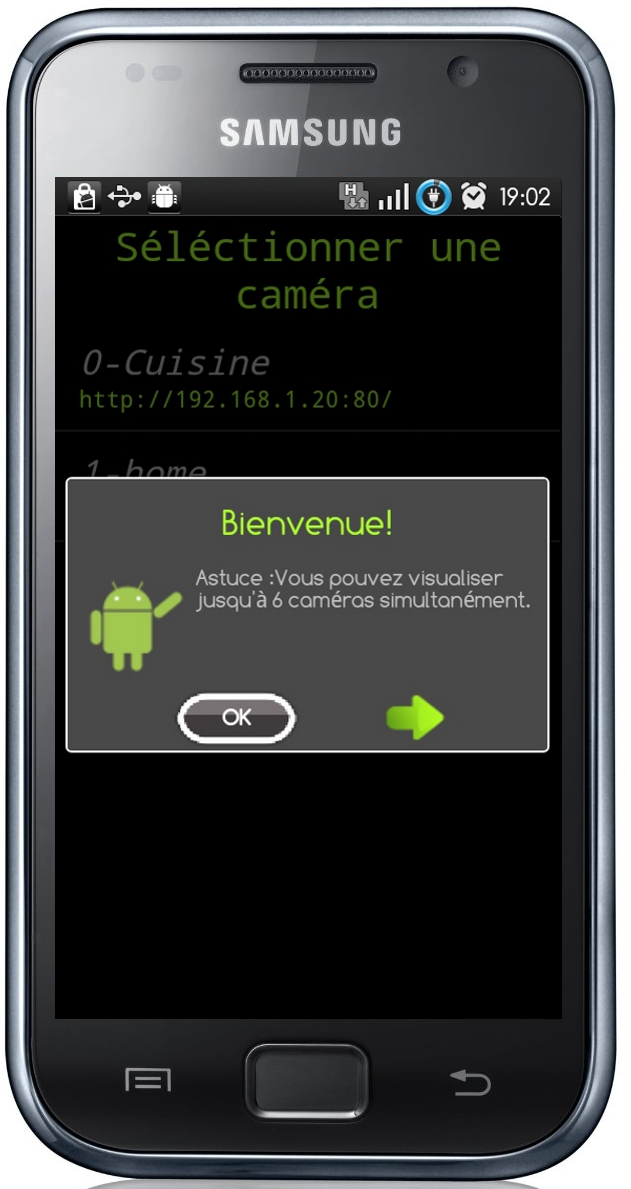
\includegraphics[width=2.5cm, height=4.5cm]{Images/ImageSlide11-3a.png}
\end{minipage}
\end{frame}
\section{Tests}
\subsection{Tests Unitaires}
  \begin{frame}
\begin{minipage}{0.32\textwidth}
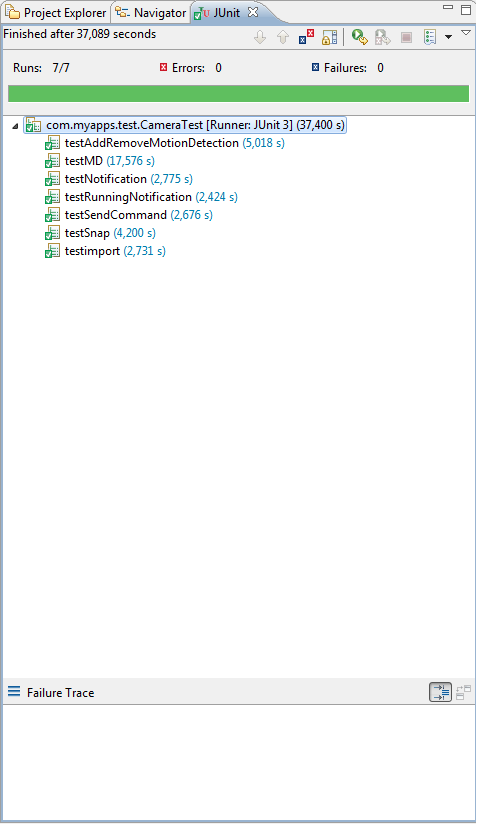
\includegraphics[width=3.5cm, height=7cm]{Images/ImageSlide12a.png}
\end{minipage}
\begin{minipage}{0.49\textwidth}
\frametitle{Tests Unitaires}
Rôle des tests unitaires
  \begin{itemize}
 \item Garantir le bon fonctionnement de l'application
    \item Vérifier si les fonctions terminent
    \item Identifier étape par étape les erreurs éventuelles
\end{itemize} 
\end{minipage}
\begin{minipage}{0.10\textwidth}
 
\includegraphics[width=3cm, height=2.2cm]{Images/ImageSlide12.png}
\end{minipage}
\end{frame}
\subsection{Tests en réel}
 \begin{frame}
\begin{minipage}{0.59\textwidth}
   \frametitle{Tests en réel}
\begin{itemize}
    \item Suivi de l'exécution en continu avec le LogCat d'Android
    \item Utilisation intensive de 3 téléphones de marques différentes
    \item Tests sur une caméra Axis PTZ 214 avec l'ensemble des
    fonctionnalités implémentées
   \end{itemize}
\end{minipage}
\begin{minipage}{0.39\textwidth}
 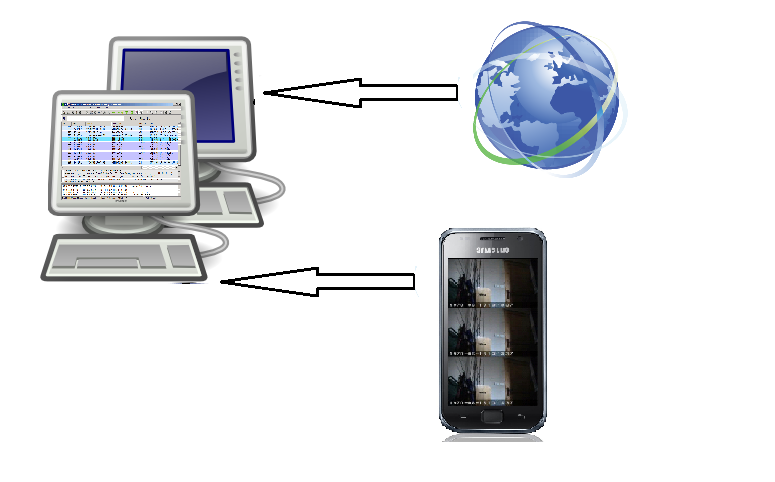
\includegraphics[width=4cm, height=3cm]{Images/ImageSlide13.png}
\end{minipage}
\end{frame}
  \begin{frame}
   \frametitle{Conclusion}
 \begin{itemize}
    \item Cahier des charges : Absence de son
    \item Application testée et opérationnelle
   \end{itemize}
 \center{
\includegraphics[width=2cm, height=2cm]{Images/ImageSlide14.png}}
\end{frame}


\end{document}